\documentclass[10pt, letterpaper]{article}
        \usepackage[utf8]{inputenc}
        \usepackage[margin=1in]{geometry}
        \usepackage{fancyhdr}
        \usepackage{titling}
        \usepackage{enumitem}
        \usepackage{mathtools}
        \usepackage{amssymb}
        \usepackage{xfrac}
        \usepackage{booktabs}
        \usepackage{graphicx}
        \usepackage{wrapfig, blindtext}
        \usepackage{hyperref}
        \usepackage{enumerate}
        \usepackage{multicol}

        
        \setlength{\parindent}{0pt}

\title{Journal 2}
        \author{Sudhan Chitgopkar}
        \date{\today}
        
        % headers -- no need to change
        \pagestyle{fancy}
        \fancyhf{}
        \lhead{OIC}
        \chead{UGAMUNC XXVII}
        \rhead{\thedate}


\begin{document}

Dear Delegates, \\

Welcome to the 27th UGA Model United Nations Conference! It is my
pleasure to be your Chair for the Organization of Islamic Cooperation
committee. My name is Roshni Saleem Chagan and I am a fourth year
student here at UGA, studying International Affairs with minors in
Spanish and English. This is my second year on the Model United Nations
team and I am extremely excited to be your Chair! When I am not doing
school work, I enjoy reading, making art, listening to music, and
drinking bubble tea! Outside of Model United Nations, I am the Vice
President for Refugee Outreach at UGA. \\

I invite you, the delegate, to be well read and compete to the best of
your ability at this conference. This background guide serves as a
foundation for your research, not an all-encompassing guide for
preparation for this conference. It is encouraged that you go beyond
your background guide and research your country's positions and these
topics further. That being said, I urge and expect you to be mindful of
debating responsibly, professionally, and in a culturally sensitive
manner, while also treating each delegate in the committee with respect.
I ask that you act with integrity and approach the topics of this
committee with consideration and respect. There is a zero tolerance
policy for any offensive language at this conference. I expect you to
act with utmost respect for others and the countries and issues being
debated over the course of the weekend. \\

When writing your position papers, I ask that you focus your research
and response within the scope of your country and maintain this scope
throughout the conference. Your speeches and contributions to
resolutions over the course of the weekend should align with your
country's position on the issues being debated. The resolutions that you
work to craft over the course of the weekend should reflect the work of
the Organization of Islamic Cooperation and relay its mission. I would
like to remind you that each nation competing in this committee is
equally important. Please remember that when working on resolutions, I
am looking for and valuing cooperation among each nation in attendance.
At the beginning of the conference, we will review parliamentary
procedure, but I urge you to review UGAMUNC rules and procedures on our
website: ugamunc.com. Should you have any questions prior to the
conference, please feel free to reach out to me! My email is
\texttt{\href{mailto:rsc78153@uga.edu}{{rsc78153@uga.edu}}}. Please
submit your completed position papers to me by February 1st. Once again,
if you have any questions, please feel free to reach out to me via
email. I look forward to a weekend of stimulating debate! \\

Best,\\
Roshni Saleem Chagan

\newpage
\tableofcontents
\newpage

\section{Topic A: Sectarian Violence in the Islamic Community}

\subsection{Introduction to the Topic}

Sectarian violence in the Islamic community started in the year 632 and
has existed since then. More recently, there have been deliberate
attempts by both Shia Muslims and Sunni Muslim to engage in behaviors
that risk erasure of the other. These occurrences are not solely
motivated by religion but also by political power and wealth,
incidentally making them issues that inherently concern human rights and
human rights abuses. This section highlights \textbf{some} of the main
instances in contemporary society in which sectarian violence is the
driving force of the conflict.

\subsection{Pakistan's Anti-Shia Sentiment}

The second week of September 2020 coincided with the end of Muharram, a
month in the Islamic calendar in which Muslims observe the death of
Muhammad's grandson and Ali's son, Hussain. Sunni Muslims and Shia
Muslims observe this month for the same reasons but have different
practices. Sunni Muslims have expressed discomfort with the Shia
practice of self-flagellation, a practice in which Shia Muslims hurt
themselves as a way to mourn the death of Hussain. This has led to Shia
Muslims in Pakistan being labeled as ``heretics.'' The weekend of
September 11, 2020, 30,000 demonstrators gathered in the streets of
Pakistan chanting ``heretics,'' anti-Shia slogans, and slurs at the Shia
Muslims of Pakistan. These demonstrators were supported by a Pakistani
political party, Sipah-e-Sahaba, which has deliberate ties to a
terrorist organization. The entire platform of this political party
revolves around expelling Shia Muslims in Pakistan.\footnote{\texttt{\href{https://www.mei.edu/publications/sectarian-violence-and-intolerance-pakistan\#_ftn3}{{https://www.mei.edu/publications/sectarian-violence-and-intolerance-pakistan\#\_ftn3}}}} \\

Before the mass demonstrations and anti-Shia hysteria during the last
weekend of Muharram, in 2015, Sunni gunmen boarded a bus in Karachi,
Pakistan and attacked the passengers. 40 Shia Muslims were killed and 13
were injured. However, this was not the biggest terror attack against
Shia Muslims that year, as earlier in 2015, a Sunni suicide bomber left
61 Shia Muslims dead. The Middle East institute, a Non-Governmental
Organization dedicated to studying affairs in the Middle East, has noted
that a total of 2,000 people have been killed and 3,500 people have been
injured in sectarian attacks in Pakistan over the span of five
years.\footnote{\texttt{\href{https://www.mei.edu/publications/sectarian-violence-and-intolerance-pakistan\#_ftn3}{{https://www.mei.edu/publications/sectarian-violence-and-intolerance-pakistan\#\_ftn3}}}}
A large majority of those who were victims of these attacks were members
of the Shia sect of Islam. The South Asia Terrorism Portal demonstrated
that the number of people killed and injured in sectarian attacks from
1989 through 2020 has an upward trend. They also noted that sectarian
attacks have become increasingly deadly in Pakistan and in each instance
they become more violent and deadly.\footnote{\texttt{\href{http://www.satp.org/satporgtp/countries/pakistan/database/sect-killing.htm}{{http://www.satp.org/satporgtp/countries/pakistan/database/sect-killing.htm}}}.} \\

\subsection{Sectarian Violence in Iraq}

The fall of Saddam Hussein's regime in Iraq threatened stability and the
extremely delicate democracy that was left. Stability was further
threatened when violence and tensions grew between Sunnis and shias,
further threatening the democracy of Iraq. People who held political
office failed to develop inclusive efforts to increase representation
and peace among the Sunnis and Shias.\footnote{\texttt{\href{https://carnegieendowment.org/files/iraq_sectarian_crisis.pdf}{{https://carnegieendowment.org/files/iraq\_sectarian\_crisis.pdf}}}} \\

Because of the role that the US played in encouraging and inciting
violence in Iraq, Sunni and Shia Muslims both found the need to turn to
radical armed groups to seek protection from the opposing group. In
Iraq, Sunni Muslims consider themselves and see themselves as a
``threatened minority'' but the Shia Muslims consider themselves the
``oppressed majority.'' The US occupation in 2003 gave rise to active
insurgency in areas that had a larger Sunni population. Sunni insurgents
overtime focused their efforts on attacking Shia individuals in hopes to
create chaos so that they could seize political control of Iraq. In
turn, Shia-driven attacks amounted and radical Shia leaders organized
violent responses, creating more violence between the two groups. By
2005, Iraqi people, both Sunni and Shia, were victims of regular
execution-style killings and bodies were routinely discovered around the
country. Shia mosques were attacked in Baghdad and at this point,
al-Qaeda called for increased attacks and more violent attacks against
the Shia population, urging war against the entire sect.\footnote{\texttt{\href{https://www.brookings.edu/wp-content/uploads/2016/06/1018iraq_al-khalidi.pdf}{{https://www.brookings.edu/wp-content/uploads/2016/06/1018iraq\_al-khalidi.pdf}}}} \\

\subsection{Sectarian Conflicts and the Syrian Refugee Crisis}

The Syrian Refugee Crisis is one of the world's largest refugee crises.
5.6 million Syrians are refugees, 6.2 million people are displaced
within Syria, and 12 million Syrians are in need of humanitarian
assistance. It is important to note that half of the people affected by
this refugee crisis are children.\footnote{\texttt{\href{https://www.worldvision.org/refugees-news-stories/syrian-refugee-crisis-facts}{{https://www.worldvision.org/refugees-news-stories/syrian-refugee-crisis-facts}}}} \\

While the Syrian Refugee Crisis is a human rights crisis and a refugee
crisis, it began as a sectarian conflict that resulted in civil war. The
Shia and Sunni groups oppose each other religiously and politically,
causing uprisings and tensions between the two groups. Bashar al-Assad
is a member of the Alawite community, which is a smaller sect of Shia
Islam. When a group of demonstrators protested in 2011 against
al-Assad's regime, the security detail of al-Assad began using violence
against these demonstrators and for anyone who did not support the
regime. The demonstrators were protesting for democracy because the rule
of Syria has been under the al-Assad family for generations. \\

The violence grew larger and a battle of democratic representation
turned into a civil war. The crisis has sectarian overtones because the
majority of Syrians are Sunni but al-Assad is Shia and has only ever
enacted policy that benefits Shia Muslims. The Sunni population and Shia
population saw this not as a battle between citizens and the government,
rather a battle between themselves, resulting in radicalized efforts
between both groups. The sectarian overtone of this conflict is what
contributed to the rise of the Islamic State (IS/ISIS).\texttt{\texttt{\footnote{\href{https://www.bbc.com/news/world-middle-east-26116868}{{https://www.bbc.com/news/world-middle-east-26116868}}}}} \\

\subsection{History of the Topic}

The sectarian conflicts within the Islamic community started after the
death of the Islamic Prophet, Muhammad, and still persist today. While
there definitely are countries in which Shia Muslims and Sunni Muslims
have positive relations, conversely, there are countries in which Shia
and Sunni Muslims are at points of contention with one another. Conflict
between the two sects has never really been solved and exists at
different points of time. \\

In 632, after the death of the prophet, Muhammad, the original split
between Shia and Sunni Muslims occurred. Most of the Prophet's followers
wanted the community of Muslims to decide amongst themselves to
determine who would succeed him.\footnote{\texttt{\href{https://www.npr.org/sections/parallels/2007/02/12/7332087/the-origins-of-the-shiite-sunni-split\#:~:text=The\%20original\%20split\%20between\%20Sunnis,Muhammad\%2C\%20in\%20the\%20year\%20632}{{https://www.npr.org/sections/parallels/2007/02/12/7332087/the-origins-of-the-shiite-sunni-split\#:\textasciitilde:text=The\%20original\%20split\%20between\%20Sunnis,Muhammad\%2C\%20in\%20the\%20year\%20632}}}}
However, there was a small group of Muslims who believed that someone
from Muhammad's family should succeed him. This small group was the Shia
Muslims who believed that Ali, the Prophet's son-in-law, should succeed
him. \\

Ultimately, the Sunni Muslims prevailed and were able to choose a
successor to be the first caliph.\footnote{A caliph is the head Islamic
  political, civil, and religious ruler.} The Shia community was upset
that the Sunnis outnumbered them and were able to choose the caliph and
the Sunnis were upset at the fact that the Shias were upset. Eventually,
violence and conflict broke out and two of the earliest caliphs were
murdered. When Ali, the man who the Shia Muslims originally wanted to
succeed the Prophet, was chosen as the fourth caliph, war erupted among
the two sects of Muslims and he was killed in 661 near the town of Kufa,
present-day Iraq. The amount of violence and war divided the Muslim
community into two divisions that would never reunite. \\

Conflict between the two groups continued well after Ali's death, when
Ali's son, Hussein, was chosen to lead the Shias. Hussein rejected the
rule of the present caliph and encouraged 72 members of his family and
friends to unite with him and fight against the Arab army of the present
Sunni caliph. This conflict is more prominently known as the Battle of
Karbala, a fight which ultimately led to the massacre of Hussein and his
72 supporters. Hussein was violently killed by decapitation and his head
was carried in tribute to the caliphate in Damascus, Syria. \\

Despite their differences, Sunni and Shia Muslims have lived in relative
peace for the most part of history, but starting in the 20th century,
the schism between the two deepened severely. Many scholars attribute
this to the fact that people were becoming more politically aware in
these spaces. This resulted in many Sunnis and Shias in the Middle East
using their politically-charged views of religion for religious and
political supremacy over one another. It was no longer about who would
lead the religious community, but which member of which sect would
possess political power. \\

The rise of the Safavid dynasty forcefully transformed the religious
salience of Iran from being a Sunni-centric country to being a
Shia-centric country. The Safavid Sufi Order essentially used religious
poetry and literature to transform the country. This poetry and
literature would later be used as religious and political
propaganda.\footnote{\texttt{\href{https://courses.lumenlearning.com/atd-tcc-worldciv2/chapter/safavid-empire/}{{https://courses.lumenlearning.com/atd-tcc-worldciv2/chapter/safavid-empire/}}}}
The Safavid rule played an integral role in inciting hatred among the
two groups because of the force they used to expel Sunnism. Another
historical event that contributed to a deeper schism between the two
groups was the Islamic Revolution in Iran of 1979. The Islamic
Revolution of Iran brought together people of Iran to oppose Mohammad
Reza Shah's role in the White Revolution, which essentially was a
modernization program that empowered only the rich people of Iran,
causing concerns of human rights violations and disruptions in rural
economies of Iran. Eventually, the youth of Iran came together and
protested the regime.\footnote{\texttt{\href{https://www.britannica.com/event/Iranian-Revolution}{{https://www.britannica.com/event/Iranian-Revolution}}}}
The protests were violent until martial law was imposed. The Prime
Minister, Shahpur Bakhtiar went into hiding and found exile in France,
prompting Ayatollah Ruhollah Khomeini to establish Iran as an Islamic
Republic, destroying the monarch's rule. \\

The Safavid Empire's rule and the Islamic Revolution of Iran played
immense roles in radicalizing a brand of Shia Islam that clashed heavily
with conservative Sunni Muslims in Saudi Arabia and eventually in other
countries following.\footnote{\texttt{\href{https://www.history.com/news/sunni-shia-divide-islam-muslim}{{https://www.history.com/news/sunni-shia-divide-islam-muslim}}}}
The Sunni-Shia schism fueled civil war in Syria, fighting in Lebanon,
and tensions in Iran, Iraq, and Yemen. Both sides, Sunni and Shia, were
guilty of using threats of terrorism against one another. Conversely,
there are many more Muslim-majority countries that have populations of
Sunni and Shia Muslims that coexist in peace, proving that these
tensions and struggles are not fueled by religion, but wealth and power. \\

\subsection{Vocabulary}

\begin{itemize}
\item
  
  \textbf{Ali:} Muhammad's son-in-law and also the man nominated by Shia
  Muslims to succeed Muhammad
  
\item
  
  \textbf{Cleric:} A religious leader
  
\item
  
  \textbf{Hussain:} Ali's son who succeeded Ali and was killed in the
  Battle of Karbala
  
\item
  
  \textbf{Muhammad:} last prophet of Islam
  
\item
  
  \textbf{Safavid Dynasty:} a ruling dynasty in Iran most known for
  establishing Shia Islam as the official religion of Iran, operated in
  the 16th-18th centuries
  
\item
  
  \textbf{Schism:} divisions between two opposing parties
  
\item
  
  \textbf{Sectarian:} concerning different sects of one thing
  
\item
  
  \textbf{Shia Muslims:} Muslims who believed that someone related to
  Muhammad should become successor
  
\item
  
  \textbf{Sunni Muslims:} Muslims who believed that someone within the
  community should succeed Muhammad as leader of the religion
  
\end{itemize}

\subsection{Sectarian Violence and its Relevance to the International
Community}

The current efforts to address sectarian violence have been limited. The
United Nations Office on Genocide Prevention and the Responsibility to
Protect has issued a a plan of action to address sectarian violence in
communities. The United Nations has also proposed something called the
``Fez Process'' in which religious leaders, members of the United
Nations, clerics, and government officials united to discuss problems
within religious communities and find ways to solve them before they
lead to human rights abuses. \\

The OIC specifically has curated its membership terms and its charter to
ensure that member states are inclusive of different sects of Islam and
have terms of treating members of the organization and the communities
they represent with fairness. The OIC charter has also set up penalties
and consequences that member states will face if they are unable to
control sectarian violence within their own communities.\footnote{\texttt{\href{https://www.globalgovernancewatch.org/library/doclib/20140815_OICMemo5.pdf}{{https://www.globalgovernancewatch.org/library/doclib/20140815\_OICMemo5.pdf}}}}
Though this may be what is written in the charter, the OIC has
traditionally remained extremely neutral and complacent in issues. The
OIC also remained silent in 2016 when a prominent Shia cleric, Sheikh
Nimr al-Nimr was executed in Riyadh, Saudi Arabia.\footnote{\texttt{\href{https://www.wilsoncenter.org/publication/the-iran-saudi-arabia-conflict-and-its-impact-the-organization-islamic-cooperation}{{https://www.wilsoncenter.org/publication/the-iran-saudi-arabia-conflict-and-its-impact-the-organization-islamic-cooperation}}}}

\subsection{How has the OIC handled this issue or issues similar?}

The OIC has handled a similar issue. They met to deliberate over the
conflict between Iran and Saudi Arabia. Iran is a Shia majority state
and Saudi Arabia is a Sunni majority state. Saudi Arabia also considers
itself as the leading Muslim power, causing inherent tensions among
itself and other Islamic nations. The two nations are neighbors, causing
there to be border tensions and regional struggles, both of which Iran
ends up winning.\footnote{\texttt{\href{https://www.bbc.com/news/world-middle-east-42008809}{{https://www.bbc.com/news/world-middle-east-42008809}}}}Though
the issue was brought to the attention of OIC member states, when Saudi
Arabia isolated Iran, it just proved to deepen the sectarian rifts
within the OIC. The OIC did not hold Saudi Arabia accountable for its
actions of violence against Iran, causing there to be a bigger rift and
also causing distrust among the Shia community and the OIC. Shia Muslims
now question the OIC's independence and ability to stand in solidarity
with all Muslims, not just Sunni Muslims. This has also been identified
as a gap of credibility between practices and ideals of the
OIC.\footnote{\texttt{\href{https://www.wilsoncenter.org/publication/the-iran-saudi-arabia-conflict-and-its-impact-the-organization-islamic-cooperation}{{https://www.wilsoncenter.org/publication/the-iran-saudi-arabia-conflict-and-its-impact-the-organization-islamic-cooperation}}}} \\

\subsection{Driving Questions}

\begin{itemize}
\item
  
  How would social welfare and community empowerment play a role in
  Pakistan's sectarian conflict?
  
\item
  
  How does the political system of a state play a role in the existence
  of sectarian violence?
  
\item
  
  How can the OIC remain objective and bridge the communication gap
  between Shia and Sunni majority countries respectively?
  
\item
  
  What concrete efforts can the United Nations take to combat sectarian
  violence?
  
\item
  
  Think about how political elitism plays a role in religious elitism.
  More specifically, consider how clerics may retain religious and
  political influence within their communities.
  
\end{itemize}

\subsection{Suggested Readings}

\begin{itemize}
\item
  
  \texttt{\href{https://www.mei.edu/publications/sectarian-violence-and-intolerance-pakistan\#_ftn3}{{https://www.mei.edu/publications/sectarian-violence-and-intolerance-pakistan\#\_ftn3}}}
  
\item
  
  \texttt{\href{https://www.history.com/news/sunni-shia-divide-islam-muslim}{{https://www.history.com/news/sunni-shia-divide-islam-muslim}}}
  
\item
  
  \texttt{\href{https://carnegieendowment.org/files/iraq_sectarian_crisis.pdf}{{https://carnegieendowment.org/files/iraq\_sectarian\_crisis.pdf}}}
  
\item
  
  \texttt{\href{https://www.brookings.edu/wp-content/uploads/2016/06/1018iraq_al-khalidi.pdf}{{https://www.brookings.edu/wp-content/uploads/2016/06/1018iraq\_al-khalidi.pdf}}}
  
\end{itemize}

\newpage
\section{Topic B: Armenia and Azerbaijan, the Nagorno-Karabakh Conflict}

\subsection{Introduction to the Topic}

Armenia announced a declaration of Martial Law on September 27, 2020.
The enactment of martial law mobilized the Aremenian army and ordered
civilians to seek shelter. Armenia announced martial law because they
had reason to believe that their neighboring country, Azerbaijan,
launched a military operation into Nagorno-Karabakh. This region is
internationally recognized as territory belonging to Azerbaijan, but
most of its population is Armenian who have lived under the rule of
Azeris for more than a century. Nagorno-Karabakh has been a point of
contention for both Azeris and Armenians but in the past two years,
there have been possible and progressive peace talks. Though relative
peace existed for some time, conflict erupted again on September 27,
2020, causing Aremenian military, Azerbaijani troops and the
Nagorno-Karabakh forces to fight with one another. This fighting has
resulted in the death of 400 civilians and hundreds were left injured.
Azerbaijan claims to have seized the Nagorno-Karabakh territory while
Armenians believe this could not be further from the truth.\footnote{\texttt{\href{https://www.theguardian.com/world/2020/sep/28/why-are-armenia-and-azerbaijan-fighting-what-are-implications}{{https://www.theguardian.com/world/2020/sep/28/why-are-armenia-and-azerbaijan-fighting-what-are-implications}}}} \\

In 2018, the Armenian Revolution ushered new leadership efforts in the
country in hopes that the Nagorno-Karabakh conflict would move towards
some sort of revolution. Armenia's prime minister, Nikol Pashinyan, took
a firm stance on the issue instead of discussing and debating with
Azerbaijan. The pandemic took a toll on Azerbaijan's oil and gas
economy, they sought territorial gains as a way to absolve themselves of
that. Azerbaijan entered the territory under the claims that it is
responding to Armenian aggression in areas that are legally the
territories of Azerbaijan. These territories have been historically
occupied by enemy troops and separatists.\footnote{\texttt{\href{https://www.theguardian.com/world/2020/sep/28/why-are-armenia-and-azerbaijan-fighting-what-are-implications}{{https://www.theguardian.com/world/2020/sep/28/why-are-armenia-and-azerbaijan-fighting-what-are-implications}}}} \\

On September 27, Armenia claimed that Azerbaijan's military was
instructed to bomb civilian settlements in the Nagorno-Karabakh
territory. In response to their actions, Armenia's defense ministry
claimed to have downed two Azerbaijani military helicopters and three
drones in response to the civilian bombings. In response to Armenia's
claims, Azerbaijan's defense ministry announced that it had launched a
``counteroffensive'' attack with tanks, war plans, missiles, and drones
into the Nagorno-Karabakh territory. \\

\subsection{History of the Topic}

Nagorno-Karabakh is a landlocked religion inside the official borders of
Azerbaijan. However, regardless of its location inside Azeri territory,
the population is mostly made up of Aremnians. The territory is both
populated and controlled by ethnic Armenians and is considered to be
extremely militarized. This has been a source of contention since before
the Soviet Union was created. Tensions were at bay when Armenia and
Azerbaijan were Soviet states but as soon as Communism fell, tensions
re-emerged. \\

In 1994, a war between Armenia and Azerbaijan ended in a ceasefire and
resulted in Armenia retaining control of the Nagorno-Karabakh territory
along with certain enclaves of territory located within Azerbaijan.
Azerbaijan is a Muslim-majority country and Armenia is a
Christian-majority country, adding an angle of religion into this
conflict but this also becomes convoluted when discussing Azerbaijan's
relationship and support of Israel.\footnote{\texttt{\href{https://www.theguardian.com/world/2020/sep/28/why-are-armenia-and-azerbaijan-fighting-what-are-implications}{{https://www.theguardian.com/world/2020/sep/28/why-are-armenia-and-azerbaijan-fighting-what-are-implications}}}}
While Azerbaijan maintains strong defense ties to Israel, Armenia is
backed by the Russian army. Russia and Turkey are on opposing sides of
this issue. Turkey has maintained support for its ally, Azerbaijan.
Erdogan, the Turkish President, believes that Azerbaijan should retain
control over the area and has pledged to support the country in
whichever way it needs to be supported during this conflict. Russia is a
consistent supporter of Armenia in both weapons and diplomacy. Tensions
between Russia and Turkey are escalating as well because of the way
Turkey has been imposing its will under the former Soviet-controlled
area. Conversely, Putin has a strong relationship with the Azerbaijani
president, Ilham Aliyev.\footnote{\texttt{\href{https://www.cnn.com/2020/09/28/europe/azerbaijan-armenia-clashes-explainer-intl/index.html}{{https://www.cnn.com/2020/09/28/europe/azerbaijan-armenia-clashes-explainer-intl/index.html}}}} \\

\subsection{Relevance to the International Community}

Turkey, according to multiple international actors and sources, has
worsened matters by arming Azerbaijan and expressing that they will back
the country regardless of its stances. Turkey has actively been seeking
more influence in the region by fully backing its ally, Azerbaijan.
Turkey and Azerbaijan share ties because of the Turkic ethnic minority
that exists in Azerbaijan. Turkey has fully backed Azerbaijan and has
explained that it will back Azerbaijan in whatever capacity is
necessary.\texttt{\footnote{\href{https://www.vox.com/21507583/armenia-azerbaijan-nagorno-karabakh-explained}{{https://www.vox.com/21507583/armenia-azerbaijan-nagorno-karabakh-explained}}}}
Weapons and training, specifically 1,000 Syrian fighters to aid
Azerbaijan in case a war erupts.\footnote{\texttt{\href{https://www.theguardian.com/world/2020/oct/02/syrian-recruit-describes-role-of-foreign-fighters-in-nagorno-karabakh}{{https://www.theguardian.com/world/2020/oct/02/syrian-recruit-describes-role-of-foreign-fighters-in-nagorno-karabakh}}}} \\

Russia possesses a formal military alliance with Armenia but also
maintains close relations with Azerbaijan, as both of the countries
existed under Soviet influence before Communism fell. Russia, France,
and the United States delegated the diplomatic processes between the two
sides, encouraging both to come to an agreement about the
issue.\footnote{\href{https://www.state.gov/joint-statement-calling-for-a-ceasefire-in-nagorno-karabakh/}{{https://www.state.gov/joint-statement-calling-for-a-ceasefire-in-nagorno-karabakh/}}}
France, the United States, and Russia have all said that both Armenia
and Azerbaijan should exercise restraint.\footnote{\href{https://www.vox.com/21507583/armenia-azerbaijan-nagorno-karabakh-explained}{{https://www.vox.com/21507583/armenia-azerbaijan-nagorno-karabakh-explained}}} \\

The United States State Department has urged both sides to cease
hostilities and use direct communication links to avoid further
escalation of conflict. Iran has called for an immediate end to the
conflict and has also decided that it is ready to help establish a
ceasefire. Turkey, as mentioned before, has decided to fully support
Azerbaijan in any capacity.\footnote{\texttt{\href{https://www.aljazeera.com/news/2020/9/27/armenia-azerbaijan-clashes-world-reactions}{{https://www.aljazeera.com/news/2020/9/27/armenia-azerbaijan-clashes-world-reactions}}}}
While the United Nations has not taken official action to mitigate
conflict, the Secretary General has voiced extreme concerns and has
called on both sides to immediately stop fighting.\footnote{\texttt{\href{https://twitter.com/UN_Spokesperson/status/1310292951256518658?ref_src=twsrc\%5Etfw\%7Ctwcamp\%5Etweetembed\%7Ctwterm\%5E1310292951256518658\%7Ctwgr\%5Eshare_3\%2Ccontainerclick_1\&ref_url=https\%3A\%2F\%2Fnews.un.org\%2Fen\%2Fstory\%2F2020\%2F09\%2F1073992}{{https://twitter.com/UN\_Spokesperson/status/1310292951256518658?ref\_src=twsrc\%5Etfw\%7Ctwcamp\%5Etweetembed\%7Ctwterm\%5E1310292951256518658\%7Ctwgr\%5Eshare\_3\%2Ccontainerclick\_1\&ref\_url=https\%3A\%2F\%2Fnews.un.org\%2Fen\%2Fstory\%2F2020\%2F09\%2F1073992}}}}

\subsection{Vocabulary:}

\begin{itemize}
\item
  
  \textbf{Communism:} political ideology in which property is publicly
  owned and each person works and is paid according to their abilities
  and needs
  
\item
  
  \textbf{Enclaves:} a portion of territory that is surrounded by a
  larger territory whose inhabitants are ethnically distinct
  
\item
  
  \textbf{Nagorno-Karabakh:} a landlocked region in Azerbaijan that has
  an ethnic-Armenian population
  
\end{itemize}

\subsection{How has the OIC handled this issue or issues similar?}

The OIC has actively condemned Armenia's attack on Azerbaijan and has
called for a politically-driven solution to the conflict at
hand.\footnote{\texttt{\href{https://www.aa.com.tr/en/asia-pacific/oic-condemns-armenias-attacks-on-azerbaijan/1988811}{{https://www.aa.com.tr/en/asia-pacific/oic-condemns-armenias-attacks-on-azerbaijan/1988811}}}}
They have however actively involved themselves in territorial disputes,
namely in the Philippines after the 1964 insurrection.\footnote{\texttt{\href{https://www.brookings.edu/wp-content/uploads/2016/06/Sharqieh-November-2012-OIC.pdf}{{https://www.brookings.edu/wp-content/uploads/2016/06/Sharqieh-November-2012-OIC.pdf}}}}
The OIC also played a role in the Yemen Conflict, but has received
severe backlash for the role it played. Many started questioning the
credibility of the OIC because of its eagerness to take a
side.\footnote{\texttt{\href{https://moderndiplomacy.eu/2019/09/13/yemen-conflict-and-oic-the-role-of-the-powerful-states/}{{https://moderndiplomacy.eu/2019/09/13/yemen-conflict-and-oic-the-role-of-the-powerful-states/}}}}

\subsection{Driving Questions}

\begin{itemize}
\item
  
  How can the OIC assist the ethnic-Armenians in Azerbaijani territory
  preserve their culture?
  
\item
  
  What role does the OIC play in potential erasure of an entire ethnic
  group?
  
\item
  
  What can the OIC do to preserve Islamic values of Azerbaijan while
  also reaching a solution that is reflective of the wants and needs of
  Armenia?
  
\item
  
  Consider how the outcome of this committee can impact aspects such as
  education, food security, and healthcare access for ethnic-Armenians.
  
\end{itemize}

\subsection{Suggested Readings}

\begin{itemize}
\item
  
  \texttt{\href{https://www.theguardian.com/world/2020/sep/28/why-are-armenia-and-azerbaijan-fighting-what-are-implications}{{https://www.theguardian.com/world/2020/sep/28/why-are-armenia-and-azerbaijan-fighting-what-are-implications}}}
  
\item
  
  \texttt{\href{https://www.cnn.com/2020/09/28/europe/azerbaijan-armenia-clashes-explainer-intl/index.html}{{https://www.cnn.com/2020/09/28/europe/azerbaijan-armenia-clashes-explainer-intl/index.html}}}
  
\item
  
  \texttt{\href{https://www.vox.com/21507583/armenia-azerbaijan-nagorno-karabakh-explained}{{https://www.vox.com/21507583/armenia-azerbaijan-nagorno-karabakh-explained}}}
  
\item
  
  \texttt{\href{https://www.aljazeera.com/news/2020/9/27/armenia-azerbaijan-clashes-world-reactions}{{https://www.aljazeera.com/news/2020/9/27/armenia-azerbaijan-clashes-world-reactions}}}
  
\end{itemize}

\newpage
\section{Topic C: The Yemen War}

\subsection{Introduction to the Topic:}

The United Nations has deemed the events that are taking place in Yemen
as, ``the world's worst humanitarian crisis.''\footnote{\texttt{\href{https://unfoundation.org/what-we-do/issues/peace-human-rights-and-humanitarian-response/yemen-a-brief-background/}{{https://unfoundation.org/what-we-do/issues/peace-human-rights-and-humanitarian-response/yemen-a-brief-background/}}}} \\

The crisis has multiple parties involved. The Houthi movement championed
cultural and religious revivalism among the Zaidi Shia Muslims in
northern Yemen. The Sunni Muslims are the majority in Yemen, leaving the
Zaidis as an extreme minority within the population. However, the Zaidi
Muslims are concentrated predominantly in the northern highlands along
the border of Saudi Arabia. \\
\begin{wrapfigure}{l}{0pt}
\centering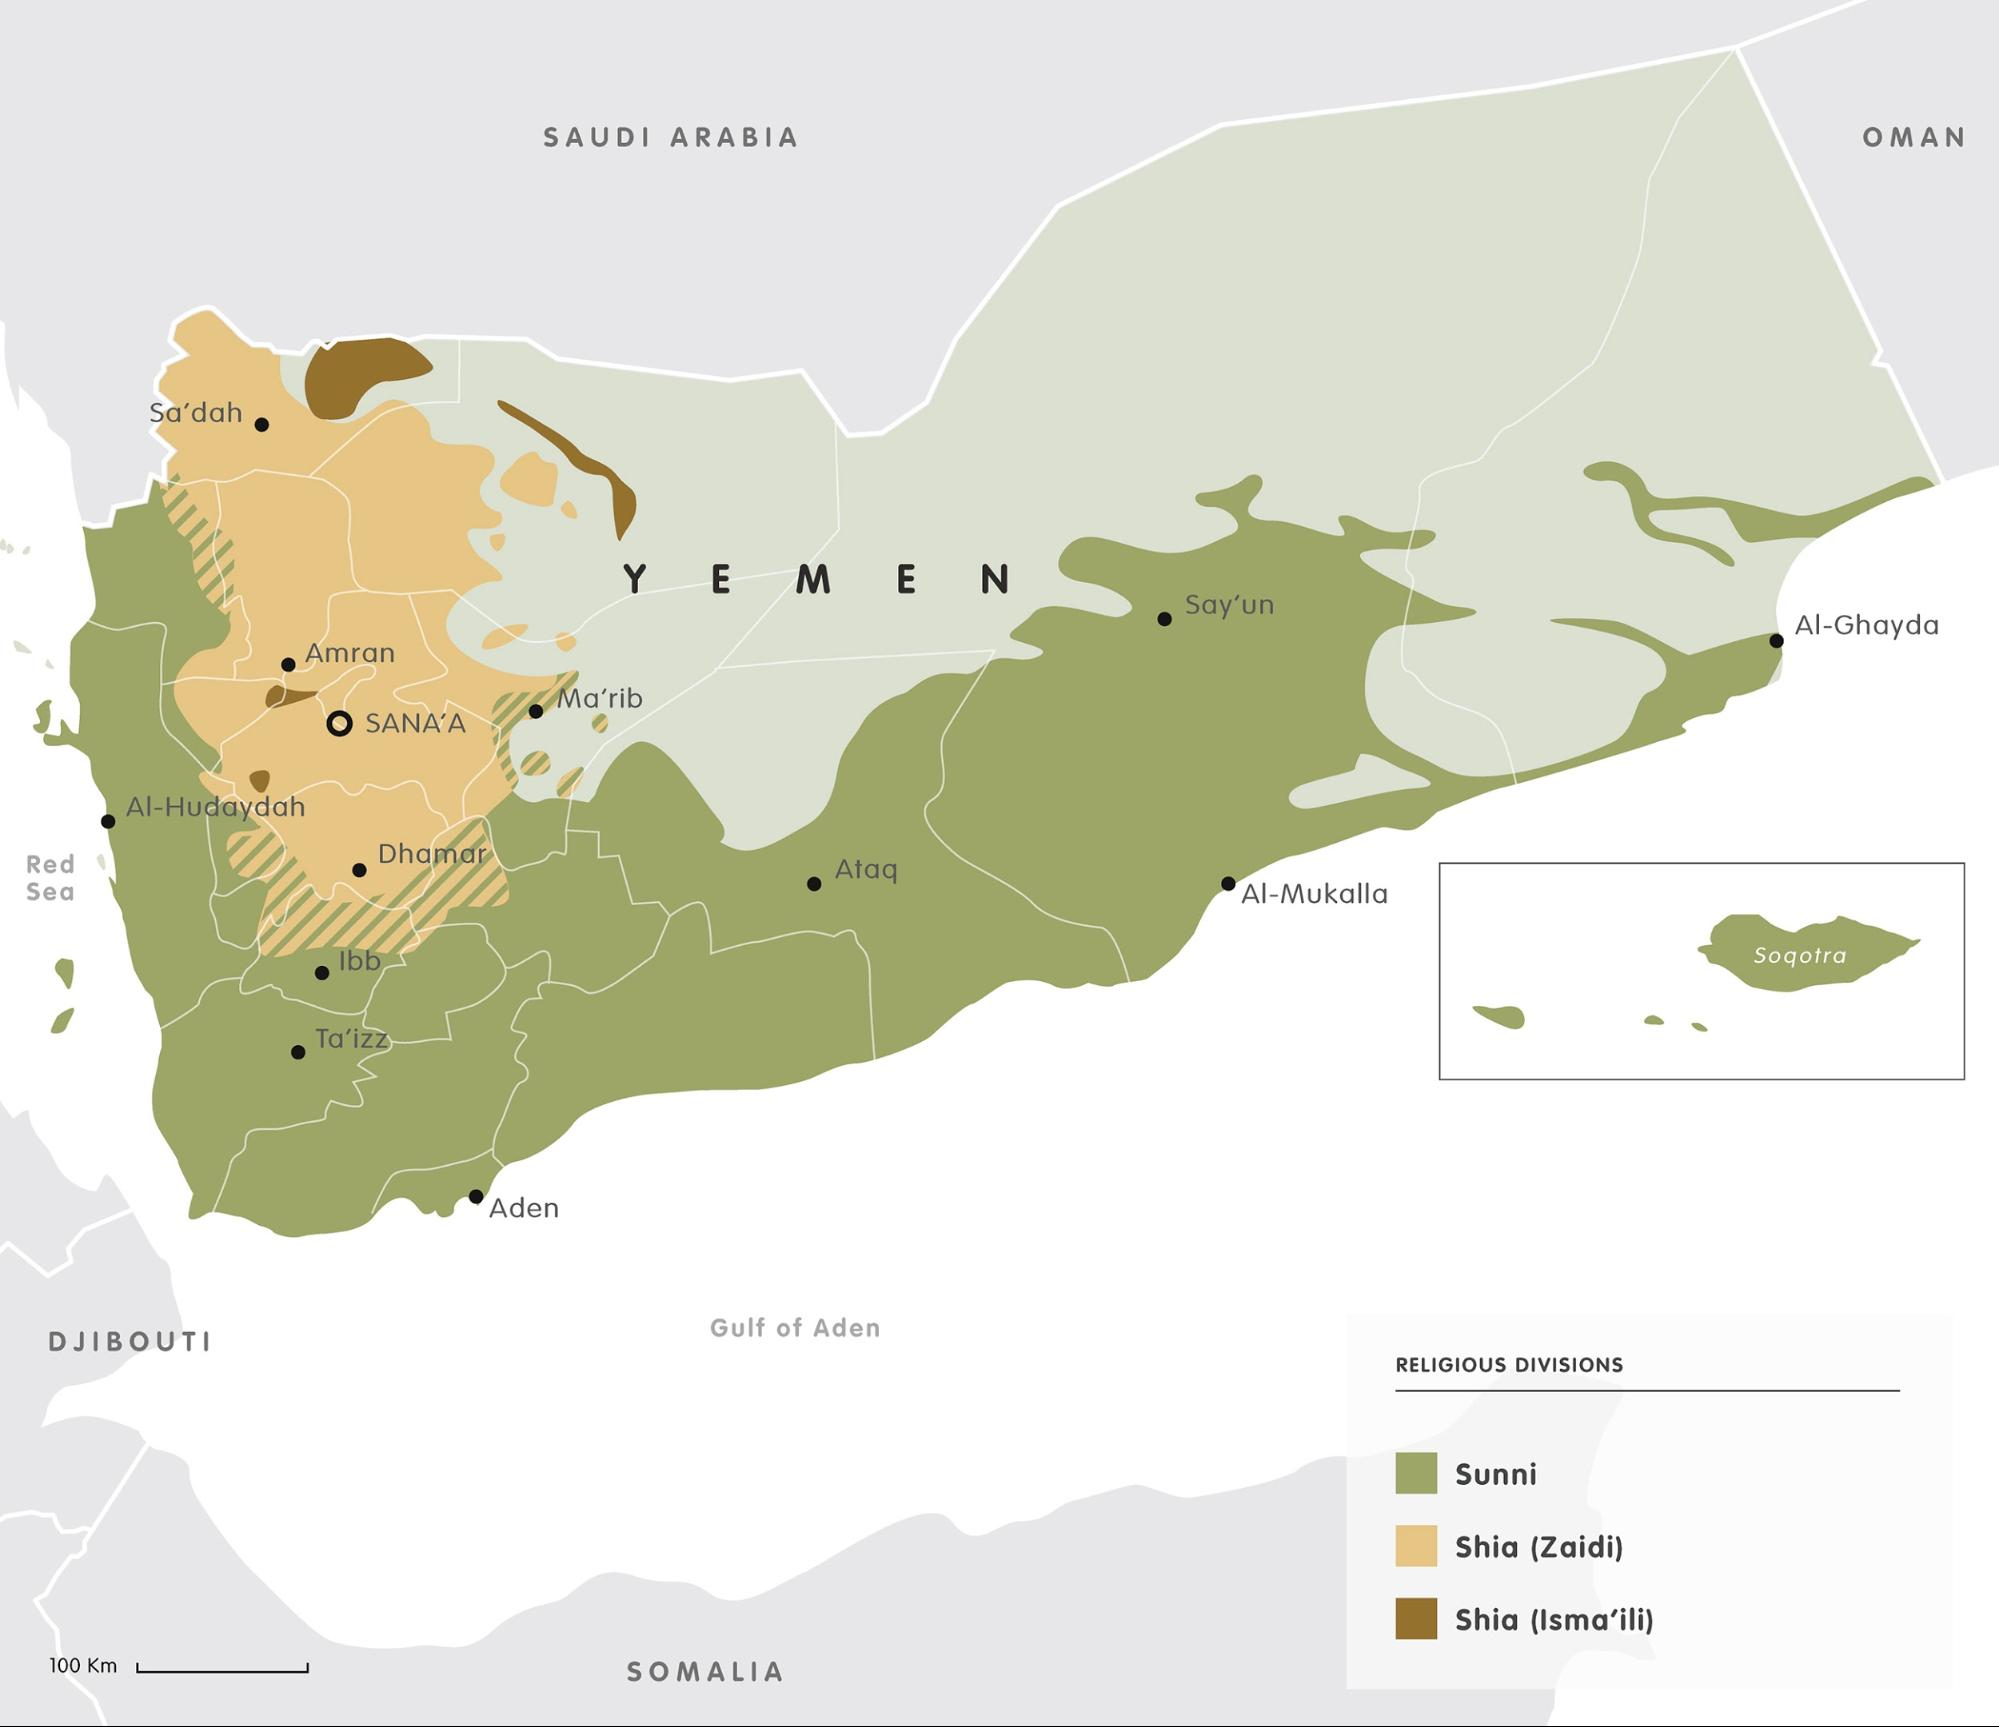
\includegraphics[scale = 0.1]{image1.jpg}\texttt{\footnote{\href{https://www.ecfr.eu/mena/yemen}{{https://www.ecfr.eu/mena/yemen}}}} \\
\caption{Zaidi Shia Muslims Concentration}
\end{wrapfigure}


The situation in Yemen has been dubbed a ``proxy war'' among many actors
on the international stage. A civil war has broken out and claimed more
than 17,500 lives in Yemen, has left 13 million people to the brink of
starvation and has left 20 million people to experience food insecurity.
Yemen is not only facing a civil war but also a famine as a result of
it. People in Yemen do not have access to food, water, and shelter as a
result of two groups fighting on behalf of Saudi Arabia and
Iran.\footnote{\texttt{\href{https://www.bbc.co.uk/newsround/38317367}{{https://www.bbc.co.uk/newsround/38317367}}}}
The access to essential resources has been blocked because deliveries of
these resources have been restricted as a result of roads and buildings
being destroyed in the civil war. \\

More than 3.5 million people have been forced to flee from their homes
but because of closed airports, blocked borders, and the ongoing
pandemic, many are unable to leave the country and seek asylum, forcing
them to face and live with these problems. Essentially, this fight is
not between Yemen and another actor. Saudi Arabia and Iran are fighting
with one another over who they support to be in control over Yemen.
However, it is the Yemeni people who are being affected the most by the
actions of Saudi Arabia and Iran.\footnote{\texttt{\href{https://www.bbc.co.uk/newsround/38317367}{{https://www.bbc.co.uk/newsround/38317367}}}} \\

\subsection{History of the Topic:}

The Yemen conflict is rooted in the failure of a political transition.
An Arab Spring uprising forced the longtime authoritarian president, Ali
Abdullah Saleh, to hand over power to his deputy Abdrabbuh Mansour Hadi
in early 2011. This political transition was supposed to bring stability
to Yemen. Once assuming the role of president, Hadi struggled to address
and solve a variety of problems such as terrorist attacks, corruption,
unemployment, and food insecurity. \\

Before forced to concede his power, Saleh was confronted by Yemen's
Zaidi Shia Muslim minority. This group fought a series of rebellions
against Saleh and as soon as the transition between presidencies took
place, they capitalized off of the new president, Hadi's, weakness by
taking control of a province named Saada and neighboring areas. The
Zaidi Shia Muslim minority believes that the Saada province is their
northern heartland. Opposing groups, such as Sunnis and Houthis, decided
to gradually take over the capital of Yemen, Sanaa, in response to the
Zaidis establishing themselves in the Saada province. The Houthis and
Sunnis remain partial to Saleh whereas the Zaidis extremely disliked
him. Because of the Houthis' loyalty to Saleh, they decided to take
control of the entire country, prompting the current president, Hadi, to
flee the country in March 2015.\footnote{\texttt{\href{https://www.bbc.com/news/world-middle-east-29319423}{{https://www.bbc.com/news/world-middle-east-29319423}}}} \\

Hadi's decision to flee the country left the Houthis in practical and
legal control of the institutional legacies of Yemen. The Houthis'
leadership and control over Yemen did not go over well. A Saudi-led
military intervention in Yemen began, and one of their biggest goals was
to oust the Houthi military and reverse their military conquest of
Yemen. They ultimately wanted to restore the Hadi government and secure
Saudi Arabia's southern border to make it free from raids, air-strikes,
and interference. Though all of these factors played a role in the
escalation of the Yemen crisis today, there are several other factors
that also contributed to this humanitarian crisis. \\

Under the pressure of the International Monetary Fund, the IMF, Yemen
was extended a \$550 million loan on the promise that the country would
engage in economic reforms. The Hadi government had lifted fuel
subsidies in July of 2014, causing the Houthis to organize mass protests
in demand for lowering fuel prices and a new government. Hadi's
supporters countered the Houthis demands and efforts, resulting in
subsidy backlash to be a factor that contributed heavily to the
humanitarian crisis in Yemen. Another factor was the Houthi takeover.
The Houthis captured the capital, Sanaa, leading the Hadi government to
resign and flee the country. Military division also plays an immense
role in this conflict because the military units that remain loyal to
Saleh, indirectly loyal to the Houthis, aligned themselves with military
efforts of Houthis, which contributed to much of their success on the
battlefield. Those who were in support of the Hadi government ramped up
their calls for secession in the south of Yemen. Saudi intervention was
just another factor that escalated this conflict because of their
intervention after Hadi fled the country. Riyadh, a city in Saudi Arabia
and consequently the capital, launched a military campaign using
primarily airstrikes to push out the Houthis and restore the control of
Sanaa to the Hadi administration.\footnote{\texttt{\href{https://www.cfr.org/backgrounder/yemen-crisis}{{https://www.cfr.org/backgrounder/yemen-crisis}}}}

\subsection{Relevance to the International Community}

The United Nations Security Council adopted Resolution 2216 in April
2015. This resolution endorsed the political goals of the Saudi military
in that they wanted the Houthi military to surrender and return to the
United Nations for facilitated and moderated discussions.\footnote{\texttt{\href{https://unfoundation.org/what-we-do/issues/peace-human-rights-and-humanitarian-response/yemen-a-brief-background/}{{https://unfoundation.org/what-we-do/issues/peace-human-rights-and-humanitarian-response/yemen-a-brief-background/}}}}
The World Food Programme, the WFP, has reached 9.5 million people in
Yemen with food assistance and will expand operations to reach 12
million people a month, including the 10 million who remain at the most
risk of a famine. The WFP has also vowed to reach the 2 million people
who are ``acutely vulnerable internally displaced peoples.''\footnote{\texttt{\href{https://reliefweb.int/report/yemen/under-secretary-general-humanitarian-affairs-and-emergency-relief-coordinator-mark-13}{{https://reliefweb.int/report/yemen/under-secretary-general-humanitarian-affairs-and-emergency-relief-coordinator-mark-13}}}}
Along with the efforts of the WFP, the United Nations Security Council
has authorized the immediate deployment of its Advance Team to monitor
force withdrawals, ceasefire in Yemen, and adopting Resolution
2451.\footnote{\texttt{\href{https://www.un.org/press/en/2018/sc13643.doc.htm}{{https://www.un.org/press/en/2018/sc13643.doc.htm}}}} \\

Saudi Arabia has played an immense role in this conflict because their
military involvement has escalated this conflict further. The UAE has
also played a significant military role in this conflict when it
supplied about 10,000 ground troops in the south of Yemen to help
coalition fighters that were supplied by Eritrea, Morocco, Pakistan,
Qatar, Saudi Arabia, and Sudan.\footnote{\texttt{\href{https://www.cfr.org/backgrounder/yemen-crisis}{{https://www.cfr.org/backgrounder/yemen-crisis}}}}
The United States Congress has been divided on this matter, as the US
has backed the Saudi-led military coalition along with countries such as
France, Germany, and the United Kingdom. The US has particular interest
in this conflict because it wants stability in Yemen, secure borders
along Saudi Arabia, free passage in the Bab Al-Mandeb strait, and
Yemen's support (specifically from Sanaa) in US counterterrorism
programs.\footnote{\texttt{\href{https://fas.org/sgp/crs/mideast/R45046.pdf}{{https://fas.org/sgp/crs/mideast/R45046.pdf}}}} \\

Overall, involvement in this crisis has been substantial but not enough
to mitigate or lessen the impact of this proxy war. The crisis in Yemen
is becoming known and unfolding as the world's worst humanitarian crisis
and international action within the right capacity is what will help aid
Yemeni people and the country itself. \\

\subsection{Vocabulary:}

\begin{itemize}
\item
  
  \textbf{Zaidi Shia Muslims:} Zaidi Shias are the oldest sect of Shia
  Islam. They are a small minority focused in Yemen.
  
\item
  
  \textbf{Houthis:} group focused on empowering and centering governance
  around Zaidi Shia Islam.
  
\item
  
  \textbf{Abdrabbuh Mansour Hadi:} Yemeni politician who fled the
  country when the capital and northern region of Yemen were captured.
  
\item
  
  \textbf{Ali Abdullah Saleh:} Yemeni politician who was ousted for
  authoritarian control over the country
  
\end{itemize}

\subsection{How has the OIC handled this issue or issues similar?}

The OIC supports the end of this conflict. Even though the OIC has
expressed interest in moderating between actors and reaching an end to
this conflict, the credibility of the OIC to be able to handle this
issue has come under fire. The entire reason the OIC was created was to
mitigate conflict between Islamic countries, yet conflicts exist so
prominently among Islamic countries. The OIC vowed to be objective when
it came to issues between Sunni and Shia Muslims but now it is taking
sides in this instance, which is contributing to its failure to solve
the Yemen conflict. \\

The OIC also has to give more attention to Saudi Arabia because it is a
leading state of the Arab League and the Arab League states have a
strong bloc in the OIC. Saudi Arabia consistently abuses its religious
position in Islam to construe the actions of the OIC and other governing
bodies in a particular way. The OIC must act in accordance with the
alliances it is a part of but also do something as the second largest
intergovernmental organization in the world after the United
Nations.\footnote{\texttt{\href{https://moderndiplomacy.eu/2019/09/13/yemen-conflict-and-oic-the-role-of-the-powerful-states/}{{https://moderndiplomacy.eu/2019/09/13/yemen-conflict-and-oic-the-role-of-the-powerful-states/}}}} \\

\subsection{Driving Questions}

\begin{itemize}
\item
  
  How can the OIC maintain its position within the alliances it is a
  part of but also effectively aid Yemen?
  
\item
  
  Consider the role Saudi Arabia plays in governance in Yemen.
  
\item
  
  Consider how your assigned role will take into account religious
  boundaries and expectations when working to solve this conflict.
  
\item
  
  How can the OIC influence the Arab League to take concrete actions
  against Saudi Arabia and Iran for this humanitarian conflict.
  
\end{itemize}

\subsection{Suggested Readings}

\begin{itemize}
\item
  
  \texttt{\href{https://moderndiplomacy.eu/2019/09/13/yemen-conflict-and-oic-the-role-of-the-powerful-states/}{{https://moderndiplomacy.eu/2019/09/13/yemen-conflict-and-oic-the-role-of-the-powerful-states/}}}
  
\item
  
  \texttt{\href{https://www.bbc.co.uk/newsround/38317367}{{https://www.bbc.co.uk/newsround/38317367}}}
  
\item
  
  \texttt{\href{https://www.cfr.org/backgrounder/yemen-crisis}{{https://www.cfr.org/backgrounder/yemen-crisis}}}
  
\item
  
  \texttt{\href{https://unfoundation.org/what-we-do/issues/peace-human-rights-and-humanitarian-response/yemen-a-brief-background/}{{https://unfoundation.org/what-we-do/issues/peace-human-rights-and-humanitarian-response/yemen-a-brief-background/}}}
  
\end{itemize}

\end{document}
